\chapter{Einleitung}
\label{ch:einl}
  \section*{Vorbemerkungen}
    Ich verwende in diesem Dokument den nach Herrn Prof. Dr. H. Laue benannten \textit{Lauehaken}: Sei $n \in \N$, dann bezeichnet $\haken{n}$ die Menge $\{1, \dots ,n\}$.
    In Anlehnung an die Schreibweise $\N_0$ für die natürlichen Zahlen $\N$\todo{vereinigt}$\{0\}$ bezeichnet $\nullhaken{n}$ die Menge $\{0, \dots , n\}$.
    
    \TODO{Es werden ausschließlich Objekte im Zusammenhang mit gravitationellen Wechselwirkungen als Körper bezeichnet. In der Regel handelt es sich im Kontext dieser Arbeit
    dabei um Sonnen, allgemeiner um Himmelskörper.}
  \section{Motivation}
  \TODO{$x_i$, $x_j$ umschreiben in $x$ und $y$!}
  \label{sec:mot}
    Angeblich soll Sir Isaac Newton durch das Fallen eines Apfels die grundlegende Idee gehabt haben, dass die Mechanik des Himmels und der Erde doch die selben sein 
    könnten \citep{memoirs}. Jeder Schüler hat von dieser Geschichte gehört - und ob sie nun wahr ist oder nicht, sein Gesetz der nicht-relativistischen Gravitation ist bis
    heute eine wichtige Formel in der Physik.
    
    Seien für zwei Körper die Massen $m_1$, $m_2$ und Positionen $x_1$, $x_2$ gegeben. Dann wirkt durch die Masse $m_2$ eine Kraft $f$ auf die Masse $m_1$, die sich durch 
    \begin{equation}
      f = \gamma m_1 m_2 \frac{x_2 - x_1}{\norm{x_2 - x_1}^3_2}
      \label{eq:simple_grav}
    \end{equation}
    ergibt \citep{newton}. Dabei ist $\gamma \approx 6{,}67408*10^{-11} m^3 kg^{-1} s^{-2}$ die Gravitationskonstante \citep{graviconst} und $\norm{\cdot}_2: \R^d \to \R^d$ die 
    euklidische Norm $z \mapsto \sqrt{ \sum_{i \in \haken{d}} |z|^2 }$. Im weiteren werden die Position eines Körpers und der Körper assoziiert. 
    
    Diese Formel für zwei Körper auszurechnen stellt zunächst kein Problem dar. Von größerem Interesse für die Wissenschaft sind aber Mehrkörperprobleme, also die gravitationellen 
    Wechselwirkungen zwischen einer Menge von Körpern. Seien im folgenden also $n \in \N$ und Körper $x_1, \dots , x_n$ mit Massen $m_1, \dots , m_n$ gegeben.
    Für $i \neq j \in \haken{n}$ wirkt mit \autoref{eq:simple_grav} durch den $j$-ten Körper eine Kraft 
    \begin{equation}
      f_{ij} = \gamma m_i m_j \frac{x_j - x_i}{\norm{x_j - x_i}^3_2}
      \label{eq:multi_grav}
    \end{equation}
    beziehungsweise durch alle Körper eine kumulative Kraft
    \begin{equation}
      f_i = \sum_{\substack{j \in \haken{n} \\ j \neq i}} \gamma m_i  m_j \frac{x_j - x_i}{\norm{x_j - x_i}^3_2}
      \label{eq:sum_grav}
    \end{equation}
    auf den $i$-ten Körper \citep{wissrech}.
    Will man nun alle auftretenden Kräfte simulieren, müssen für alle $n$ Körper jeweils $(n-1)$ Gleichungen gelöst werden. Das Problem hat also eine Komplexität von
    $\mathcal{O}(n^2)$.
    
    Problematisch wird dies, wenn man sich beispielsweise die Dimensionen unseres Sonnensystems vergegenwärtigt. Laut \citet{nasa} besteht die Milchstraße aus etwa 100 Milliarden
    (also $10^{11}$) Sonnen. Für sämtliche gravitationelle Wechselwirkungen müssten also ungefähr $(10^{11})^2 = 10^{22}$ Terme gelöst werden. Geht man davon aus, dass ein aktueller 
    Prozessor nicht mehr als eine Milliarde Terme pro Sekunde ausrechnen kann, so benötigt er etwa $10^{13}$ Sekunden, also mehr als 300.000 Jahre für einen einzigen Simulationsschritt.
    Ein Problem dieser Größenordnung könnte also nicht in annehmbarer Zeit gelöst werden.\citep{wissrech} 
    
    In dieser Arbeit wird ein zweigleisiger Ansatz am vorliegenden Beispiel vorgestellt, mit dessen Hilfe Probleme dieser Größen- und Komplexitätsklasse in den Griff zu bekommen sind.
    
  \section{Ziele}
    \TODO{Der erste Schritt ist über Approximation die Komplexitätsklasse des Problems zu reduzieren. Reduktion auf O(n)}
    \TODO{In einem weiteren Schritt wird der vorige Algorithmus zur Ausführung auf Parallel-Rechner-Systemen angepasst.}
  \section{Aufbau}
    \TODO{machen}
    
    
    %TUTORIAL:
  \section{tutorial}
  \TODO{entfernen}
    Dies ist die Einleitung
    \citet{Shaw2003} haben ein ganz tolles Papier geschrieben
    Dies war ein Beispiel für den \textit{natbib} Befehl für \texttt{\textbackslash{}citet\{\}}.

    \textit{AspectJ} ist ein tolles Tool~\citep{AspectJ}. Dies war ein Beispiel für den \textit{natbib} Befehl \texttt{\textbackslash{}citep\{\}}.

    Kieker: \citep{Rohr2008, Hoorn2009, Hoorn2012}

    Artikel Beispiel: \citep{Frey2011}

    Weitere Hinweise auf \url{http://se.informatik.uni-kiel.de/research/scientific-work/} und \url{http://www.twenzel.de/}.
    
    \begin{lstlisting}[language=Java, label=lst:imabclass, caption=ImbaClass in Java code]
	public class ImbaClass {
		private static final String constantString = "I am imba";
	}
    \end{lstlisting}
    
    \begin{figure}[t]%
      \centering
      \begin{subfigure}{\textwidth}
	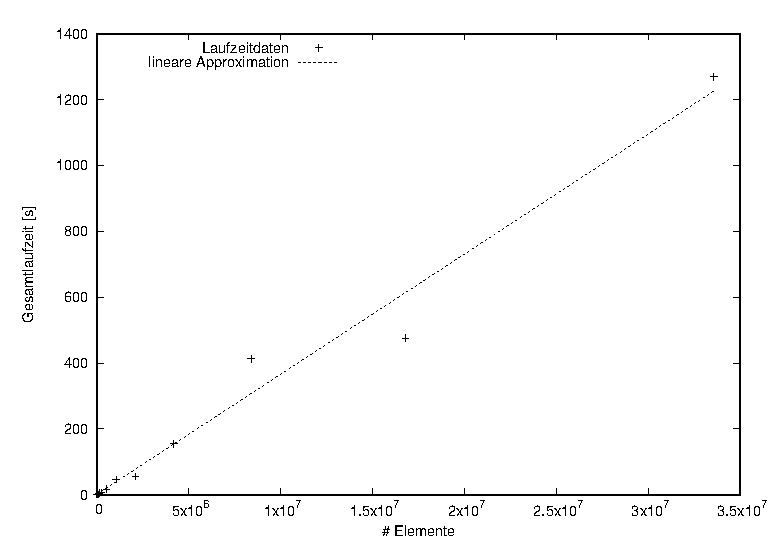
\includegraphics[width=0.9\textwidth]{img/grav_1_x_lin.eps}
	\subcaption{ }
      \end{subfigure}
      \begin{subfigure}{\textwidth}
	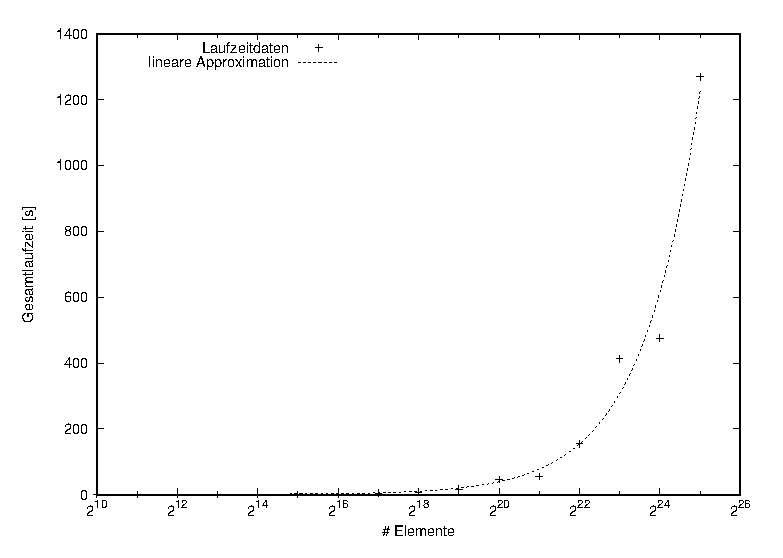
\includegraphics[width=0.9\textwidth]{img/grav_1_x_log.eps}
	\subcaption{ }
      \end{subfigure}
      \caption{muhaha}
    \end{figure}%
    